\documentclass[12pt]{article}
%Paquetes
\usepackage[left=2cm,right=2cm,top=3cm,bottom=3cm,letterpaper]{geometry}
\usepackage{lmodern}
\usepackage[T1]{fontenc}
\usepackage[utf8]{inputenc}
\usepackage[spanish,activeacute]{babel}
\usepackage{mathtools}
\usepackage{amssymb}
\usepackage{enumerate}
\usepackage{tabularx}
\usepackage{wasysym}
\usepackage{listings}
\usepackage{graphicx}
\usepackage{hyperref}
%\usepackage{graphicx}

%Preambulo
\title{Cómputo Evolutivo \\ Proyecto 1: Agente Viajero}
\author{Andrea Itzel González Vargas \\
  Carlos Gerardo Acosta Hernández}
\date{Facultad de Ciencias UNAM \\ Entrega: 07/09/16}
\begin{document}
\maketitle
\section*{Introducción}
\subsection*{Panorama general}
Como primer proyecto de la materia implementamos un Algoritmo Genético
para resolver instancias del
\textit{Problema del agente viajero} (TSP, por sus siglas en inglés),
-se consideró el caso simétrico.
Para lograrlo, utilizamos el framework de desarrollo escrito en \textit{Java}
provisto por el ayudante de laboratorio, Roberto Monroy, en las prácticas de clase.\par
Dado que el framework provee de
una estructura modularizada para el desarrollo, el código pertinente y
referente a los principios de un AG -como los procesos de selección,
cruzamiento, mutación, así como los operadores que involucran- pueden
revisarse independientemente en la carpeta de ``sources'' (src/) del proyecto.\par
Como entrada, el programa recibe un archivo con extensión \textit{.tsp},
que representa, con cierta sintáxis especial dentro de un archivo de texto plano,
una instancia del problema del agente viajero.
En el directorio del proyecto
es posible encontrar numerosas instancias\footnote{Se pueden descargar de la página del curso \href{https://sites.google.com/site/unamfcienciascomputoevolutivo/assignments/assignment1/tsp.tar.gz}{aquí}.} del problema, entre ellas las que
fueron empleadas para el análisis de resultados -burma14, ulysses16, ulysses22, gr17 y gr21.
Todas ellas se pueden revisar dentro del proyecto en el carpeta de datos (tsp/).\par
% instrucciones y github
De ser necesario, es posible leer instrucciones sobre la ejecución del programa
en el \textit{Readme} incluído en la raíz del directorio del proyecto.
También, para revisar el contenido sin necesidad de descargarlo,
se puede navegar amablemente por las líneas de código desde nuestro repositorio
alojado en \textit{GitHub}\footnote{Enlace a repositorio del proyecto: \href{https://github.com/Kihui/Proyecto-TSP}{Proyecto-TSP}}

\newpage
\subsection*{Especificación}
La implementación está basada en la solución al problema propuesta en el
libro de \textit{Algoritmos Genéticos} de Kuri-Galaviz.
\subsubsection*{Codificación del problema}
Como se comenta en el libro, hay una marcada preferencia por la utilización de
representaciones binarias para la codificación en problemas que intentan
resolver los algoritmos genéticos, principalmente porque se ven favorecidas
por los resultados del \textit{Teorema del Esquema}. Sin embargo, para este
problema en particular tiene un par de desventajas que nos llevaron a elegir
otra codificación.\par
Para empezar, una instancia del problema posee un número fijo
de ciudades que tiene que recorrer el agente viajero. Es importante procurar
representar cada una y mantener esa representación a lo
largo del algoritmo. En caso de elegir una representación binaria,
la codificación que se hace de cada ciudad requiere de ensambles binarios tan
grandes como sea necesario para representar el total de ciudades.\par
Por otro lado, ya en la ejecución del algoritmo genético, los operadores de
cruza y mutación fácilmente pueden producir ensambles de binarios que en
su decodificación no sean parte del dominio del problema, es decir, que si
cambiamos uno sólo de los bits quizá deje de existir un mapeo correspondiente con las
ciudades de la instancia. No sólo eso, también es posible que dentro de un mismo
ensamble de bits de un \textit{genotipo} resulte una ciduad repetida, lo cuál,
por definición no está permitido. Se vuelve entonces necesario implementar un
corrector que entre en juego luego de la actividad de los operadores y en la
generación de una población inicial.\par
Es por lo anterior que nos decidimos por implementar la \textbf{codificación no binaria} descrita
en el libro. Para esta codificación cada individuo es un recorrido por las ciudades
y cada alelo en su fenotipo es una ciudad, representada por un entero. De esta
manera, se asegura que los operadores sólo se manejen sin afectar la validez
de un solo alelo como en la representación binaria, entonces sólo tenemos que
preocuparnos por la validez del individuo.
Además se ajusta bastante bien a las condiciones en que recibimos las instancias de TSP,
pues cada ciudad es un nodo con un entero asociado.
La generación de una población inicial ``aleatoria'' se hace cuidando que se
generen individuos válidos, asignado sólo una vez cada ciudad a cada nuevo individuo
-puede verse de hecho como múltiples permutaciones de la lista de
ciudades en la instancia del problema.
El resto del proceso del AG se reconsideró bajo las premisas de esta representación
no binaria, por lo que los operadores no constituyen un riesgo para la validez
de los códigos genéticos ni los individuos que generan y no fue necesaria la
implementación de un corrector.

\subsubsection*{Criterio de detención}
Elegimos como criterio de detención un \textbf{número de generaciones} máximo
definido en la construcción de una instancia de nuestro Algoritmo Genético.
\subsubsection*{Evaluación de la población y Selección}
El problema del agente viajero es un problema de minimización,
como no nos es posible utilizar una traducción directa de uno de maximización,
pues al multiplicar por -1 la función de evaluación obtendremos
costos no permitidos por la definición del problema, hicimos un reajuste a
la evaluación de la población.
Primero consideramos el fitness como nuestro costo de viaje, es decir, cada
individuo representando un viaje tiene un costo asociado que es la suma de
las distancias entre sus ciudades, considerando que es un recorrido cíclico,
se suma también la distancia entre la última ciudad y la primera (sin olvidar
que la distancia es simétrica en estos problemas). Definida para un genotipo como:
\begin{equation}
  fitness(g) = d(g[0],g[n-1]) + \sum\limits_{i=0}^{n} d(g[i],g[i+1])
\end{equation}
Por conveniencia de implementación bajo el framework -pues una implementación de
la interfaz de \textit{FitnessFunction} emplea su evaluación sobre un sólo
fenotipo- se decidió que ésta fuera
el fitness, aunque se asocie más fácilmente con el concepto de \textit{función objetivo}.\par
Por otro lado, la función objetivo implementada y que para la lógica de
nuestro AG lo tratamos como función de adaptación -en el framework se aplica para una población
y por tanto resultaba más útil puesto que el grado de adaptación de un individuo
depende del resto de la población-, la definimos para un genotipo, dados los costos máximo
y mínimo de la población, como:
\begin{equation}
  evalObj(g) = (fitness_{max} + fitness_{min})-fitness(g)
\end{equation}
Señalamos que el FrameworkAG considera a los mejores y peores individuos para
un problema de maximización, por lo que aunque se señale en la interfaz gráfica
del programa una acotación verde para los mejores individuos en las estadísticas,
en realidad el individuo que nos interesa a nosotros es el de acotación color
rojo, pues es el de menor costo de viaje en la población.\par

Decidimos utilizar este remapeo de la función de adaptación con el fin de
utilizar la \textbf{selección proporcional} de ``ruleta''. La elegimos por
nuestra experiencia con la práctica anterior.
\subsubsection*{Cruza}
Para el operador de cruza, implementamos el \textbf{cruzamiento uniforme ordenado}
descrito en el libro del profesor. Con este tipo de cruzamiento nos aseguramos
de que se generen individuos válidos al aplicar el operador sobre dos individuos
de la población que hayan sido seleccionados para este proceso. Es decir,
el nuevo individuo no tendrá repeticiones de ciudades.\par
Para lograr esto se emplea una ``máscara'' de bits del tamaño del genotipo.
Como en el cruzamiento uniforme, se realiza un experimento de \textit{Bernoulli}
por cada ciudad contenida en el individuo que se reflejará en la máscara.
Para aquellos índices donde la máscara tenga valor de 1 se agregarán las ciudades
correspondientes del primer padre al nuevo individuo (en consecución) y
aquellos índices donde la máscara haya resultado con valor 0, se generará una
lista de ciudades correspondientes a esos ceros del primer padre y se agregarán
al nuevo individuo sobre los genes por asignar en el orden en que aparecen esas
ciudades dado el genoma del segundo padre.\par
Lo anterior es un mero esbozo de explicación que puede ser encontrado con más
detalle en el libro\footnote{Kuri-Galaviz, Algoritmos Genéticos, págs. 91,92} y
puede revisarse con detalle nuestra implementación en el archivo de clase
\textit{AVCrossover.java}.
\subsubsection*{Mutación}
De la misma manera que con el cruzamiento, el operador mutación está planteado
para producir un individuo ``mutado'' válido en la instancia del problema.\par
El algoritmo utilizado para esta mutación también hace uso de una ``máscara'',
una cadena de bits del mismo tamaño del individuo a mutar. Ésta se genera dada
la probabilidad de mutación $p$ en la ejecución del programa. Se establecerá entonces
un bit 1 en la máscara con probabilidad $p$ y un 0 con probabilidad $1-p$.\par
Posteriormente, para aquellos índices en que la cadena de bits tenga asignado
un 1, se generará una lista con las ciudades correspondientes del individuo y
se eliminará ese gen del individuo, después
se realizará una permutación de los elementos de esta lista de manera que
ninguno termine en la posición en que se encontraba originalmente al crearla.\par
Finalmente, en los genes vacíos del individuo se acomodarán las ciudades en el
orden que aparecen en la lista temporal que se permutó. De esta forma, no es posible
repetir ciudades, pues la mutación es básicamente una permutación de las ciudades
en el individuo original a mutar.\par
Para revisar el pseudo-código del algoritmo, igualmente puede ser encontrado en
el capítulo 3 del libro y nuestra implementación en el archivo de clase
\textit{AVMutation.java}, dentro del directorio de código fuente del proyecto.

\subsubsection*{Experimentos}
Se escogieron tres valores de probabilidad de mutación (P$_m$) y tres valores de
probabilidad de cruza (P$_c$), con las cuales se formaron todas las posibles
combinaciones de parejas dejándonos con un total de nueve parejas. \\

\noindent Se usaron los archivos burma14, ulysses16, gr17, gr21 y ulysses22, cada uno se probó
con las nueve parejas distintas y por cada una de éstas se hicieron tres experimentos
distintos, por lo que en total se hicieron 9$\times$5$\times$3 experimentos. \\

\noindent Se fijó la población en 200 individuos y se corrieron 2000 generaciones por cada
experimento. \\

\noindent Probabilidades escogidas: \\

\begin{center}
    \begin{tabular}{c | c}
      P$_c$ & P$_m$  \\ \hline
      0.6 & 0.001  \\ \hline
      0.7 & 0.051  \\ \hline
      0.8 & 0.101  \\ 
    \end{tabular}
\end{center}

\noindent Las tres mejores parejas resultaron ser aquellas donde P$_m$ es menor, i.e.
(representamos cada pareja como (P$_c$, P$_m$)) \\
(0.6, 0.001), (0.7, 0.001) y (0.8, 0.001) \\

\noindent En ésta gráfica se puede apreciar el exceso porcentual promedio de éstas  parejas
en cada generación: \\

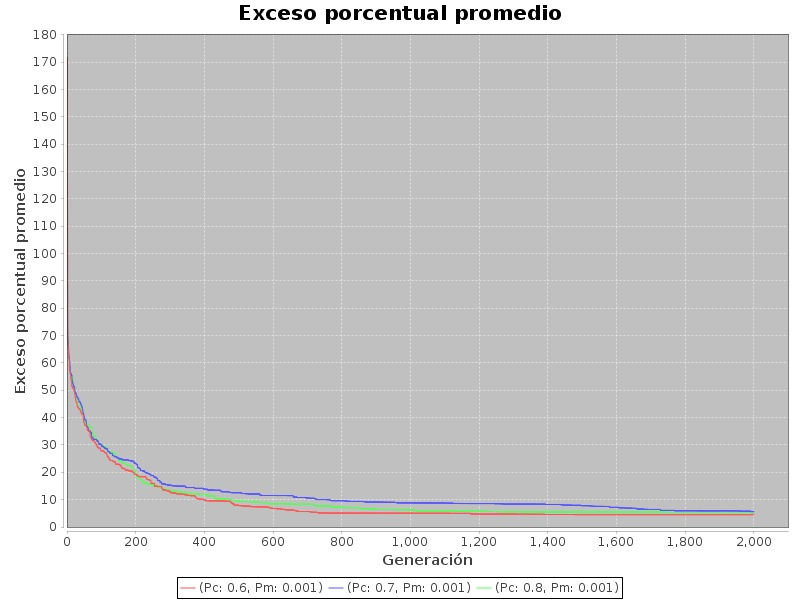
\includegraphics[width=\textwidth]{datos.jpeg} \\

\noindent Y a continuación se muestran éstos mismos datos para el resto de las parejas: \\

\begin{center}
  \begin{table}[!htbp]
  \caption{Exceso porcentual promedio por parejas}
  \begin{tabular}{| c | c | c | c | c | c | c |}
    \hline
      Generación & (0.6, 0.051)  & (0.6, 0.101)  & (0.7, 0.051)  & (0.7, 0.101)  & (0.8, 0.051)  & (0.8, 0.101)  \\ \hline
      0 & 171.67 & 171.67 & 171.67 & 171.67 & 171.67 & 171.67 \\ \hline
      100 & 28.97 & 30.63 & 29.45 & 35.49 & 34.49 & 37.13 \\ \hline
      200 & 22.48 & 23.59 & 24.18 & 28.73 & 29.49 & 29.61 \\ \hline
      300 & 17.89 & 20.19 & 20.98 & 23.40 & 25.97 & 27.55 \\ \hline
      400 & 16.36 & 18.10 & 17.74 & 20.31 & 21.50 & 24.47 \\ \hline
      500 & 13.83 & 15.22 & 16.32 & 19.00 & 20.42 & 21.57 \\ \hline
      600 & 13.38 & 14.28 & 15.73 & 16.18 & 17.58 & 20.12 \\ \hline
      700 & 11.91 & 12.53 & 15.43 & 15.47 & 16.89 & 18.63 \\ \hline
      800 & 10.78 & 12.38 & 14.78 & 15.01 & 16.28 & 17.11 \\ \hline
      900 & 10.58 & 12.34 & 13.26 & 14.40 & 15.50 & 15.09 \\ \hline
      1000 & 10.04 & 11.36 & 12.80 & 13.50 & 14.81 & 14.41 \\ \hline
      1100 & 9.53 & 11.31 & 12.55 & 12.80 & 14.38 & 13.88 \\ \hline
      1200 & 9.15 & 11.13 & 12.47 & 11.84 & 13.43 & 13.00 \\ \hline
      1300 & 8.98 & 10.94 & 11.52 & 11.72 & 13.04 & 12.82 \\ \hline
      1400 & 8.98 & 10.78 & 11.30 & 11.05 & 12.45 & 11.97 \\ \hline
      1500 & 8.79 & 10.51 & 10.68 & 10.77 & 12.33 & 11.54 \\ \hline
      1600 & 8.74 & 10.36 & 10.04 & 10.75 & 11.94 & 11.07 \\ \hline
      1700 & 8.50 & 10.31 & 10.03 & 10.46 & 11.73 & 10.85 \\ \hline
      1800 & 8.50 & 10.31 & 9.77 & 10.10 & 11.17 & 10.22 \\ \hline
      1900 & 8.30 & 10.29 & 9.26 & 9.83 & 11.10 & 10.03 \\ \hline
      2000 & 8.30 & 9.97 & 9.06 & 9.41 & 10.37 & 9.84 \\ \hline

    \end{tabular}
    \end{table}
\end{center}

\end{document}
